\section{Software Microcontrollore}
Il codice per la programmazione del microcontrollore si sviluppa dall'applicazione di base "\textit{LoRaWAN\_End\_Node}" che fornisce
le funzioni necessarie per l'inizializzazione dei componenti base per la comunicazione del microcontrollore attraverso il protocollo LoRa.
\\\\Per poter leggere i dati che si intendono acquisire dai sensori si è reso necessario organizzare e riformulare parte di codice per l'inizializzazione e il funzionamento dell'accelerometro
e del giroscopio. Nelle sezioni \ref{ssec:sensori} e \ref{ssec:lorawan} vengono rispettivamente presentate la strategia di collegamento e lettura dei sensori selezionati e 
le modifiche apportate al codice per poter comunicare correttamente con il cloud.

\subsection{Lettura sensori}\label{ssec:sensori}
% BREVE SCALETTA:
% 1) Descrizione breve del collegamento hardware e del bus I2C
Per fare in modo che il microcontrollore riceva i dati acquisiti dai sensori, è stato effettuato il collegamento hardware tra i due componenti con i pin specifici della scheda (PA11 e PA12) 
adibiti alla comunicazione attraverso bus I2C. Una volta completato questo passaggio, con l'integrazione dei driver di basso livello del sensore X-CUBE-MEMS1 si è resa possibile l'effettiva comunicazione.\\

% 2) Descrizione delle funzioni per l'inizializzazione e l' acquisizione dei sensori dall'almbiente esterno
% -Cenno a LSM6DSO_USER_Init() e la sua posizione nel codice
% -Cenno LSM6DSO_USER_Acc_GetAxes() e LSM6DSO_USER_Gyro_GetAxes()
Per leggere i dati misurati dall'accelerometro e dal giroscopio, sono state sviluppate due funzioni in particolare (riportate in Figura \ref{fig:lettura_sensori}). Queste due funzioni leggono i dati dell'accelerometro e del giroscopio rispettivamente e restituiscono un "exit code" uguale a zero se la lettura è stata completata con successo. I valori letti vengono scritti sulle tre variabili passate tramite puntatore.
\begin{figure}[h!]
  \centering
  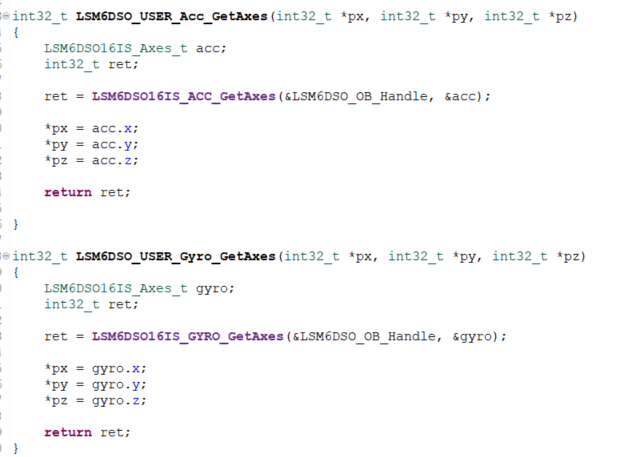
\includegraphics[width=0.75\textwidth]{getDataFunctions.png}
  \caption{Funzioni di lettura dei sensori}
  \label{fig:lettura_sensori}
\end{figure}
\\Affinché queste funzioni operino correttamente, è necessario richiamare anche altre funzioni di inizializzazione:
\begin{itemize}
  \item \Verb|LSM6DSO_USER_Init()| all'interno della funzione \Verb|LoRaWAN_Init| (dichiarata nel file \textit{lora\_app.c})
  \item \Verb|BSP_I2C2_Init()| nel \textit{main.c}
\end{itemize}
% 3) Descrizione della funzione EnvSensorRead() e della struttura dati sensor_data per la lettura del sensore
I dati che si intendono inviare al cloud sono racchiusi nella variabile \Verb|sensor_data| (presente in Figura \ref{fig:envsensorread}) di tipo \Verb|sensor_t|. La struttura di \Verb|sensor_t|, riportata in Figura \ref{fig:sensor_t} è definita nel file \textit{sys\_sensor.h} ed è stata modificata aggiungendole i campi \Verb|acc_x|, \Verb|acc_y| e \Verb|gyr_y|, necessari al funzionamento del sistema.
\begin{figure}[h!]
  \centering
  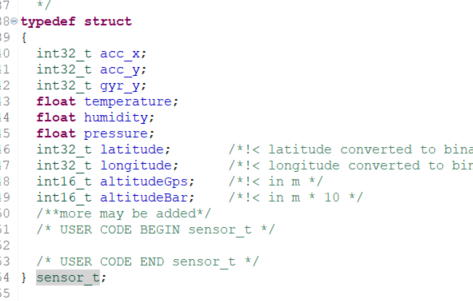
\includegraphics[width=0.7\textwidth]{sensor_t.png}
  \caption{Struttura dati sensor\_t}
  \label{fig:sensor_t}
\end{figure}
\\La funzione \Verb|EnvSensorRead| (definita nel file \textit{sys\_sensor.c} e riportata in Figura \ref{fig:envsensorread}) legge i dati dei sensori e li scrive nella variabile \Verb|sensor_data| (passata tramite puntatore). Questi dati saranno poi processati nella funzione \Verb|SendTxData| (vedi Sezione \ref{sssec:uplink_scheda}).
\begin{figure}[h!]
  \centering
  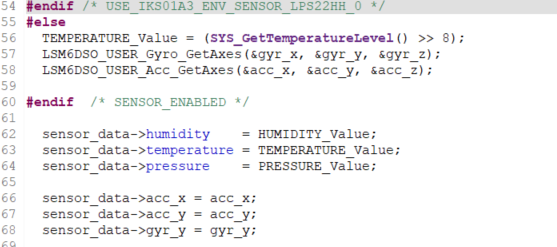
\includegraphics[width=0.8\textwidth]{EnvSensorRead.png}
  \caption{Parte della funzione EnvSensorRead}
  \label{fig:envsensorread}
\end{figure}

\subsection{LoRaWAN}\label{ssec:lorawan}
% Breve descrizione del protocollo di rete
% -LoRaWAN_Init() per l'aggiornamento delle variabili
% -Cenno al DutyCicle per il tempo di lettura delle variabili? --> 3-4s ottimale
% File utili: main.c app_lorawan.c lora_app.c
Il uC, una volta connesso ad un gateway LoRa, invia i dati al cloud ogni 10 secondi (quantità definita dalla costante \Verb|APP_TX_DUTYCICLE| nel file \textit{lora\_app.h}) e legge i dati in entrata appena vengono caricati sul cloud dal client.
\\Un'idea per ottenere un interfaccia grafica e di conseguenza un programma più performante potrebbe essere quella di abbassare il dutycicle a pochi secondi.

  \subsubsection{Uplink scheda}\label{sssec:uplink_scheda}
  % Descrizione della funzione SendTxData
  % -Riferimento a variabile roll_state per decidere che dati inviare
  % -Strategia operativa per inserire i dati di sensor_data nel buffer
  Il uC invierà al cloud i valori presenti nella variabile \Verb|AppData.Buffer|, un array di tipo \Verb|uint8_t|, i cui valori degli elementi sono definiti nella funzione \Verb|SendTxData| (all'interno del file \textit{lora\_app.c}).
  Dato che i valori letti dai sensori (\Verb|acc_x|, \Verb|acc_y| e \Verb|gyr_y|) sono di tipo \Verb|int32_t| e gli elementi del buffer sono di tipo \Verb|uint8_t|, bisogna scrivere all'interno del buffer 8 bit alla volta partendo dai più significativi. Un esempio grafico di come i dati di tipo \Verb|int32_t| vengono suddivisi è riportato di seguito in Figura \ref{fig:int32tobuffer}.
  \begin{figure}[H]
    \centering
    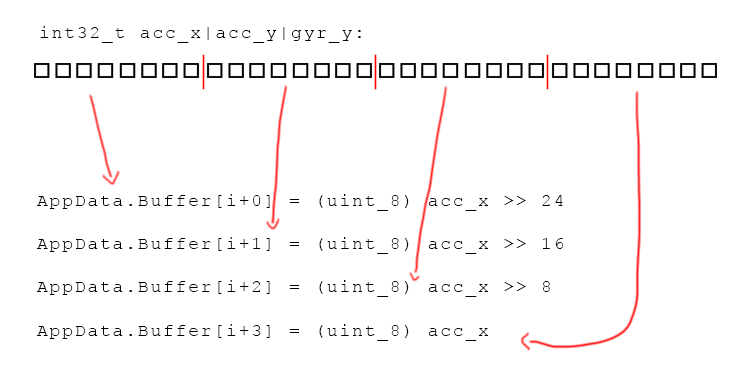
\includegraphics[width=0.9\textwidth]{spiegazione_scrittura_int32.png}
    \caption{Come valori di tipo int32\_t vengono suddivisi e scritti sul Buffer}
    \label{fig:int32tobuffer}
  \end{figure}
  Nella funzione \Verb|SendTxData| riportata in Figura \ref{fig:sendtxdata}, vengono invece definiti i valori degli elementi del buffer:\\
\begin{figure}[H]
  \centering
  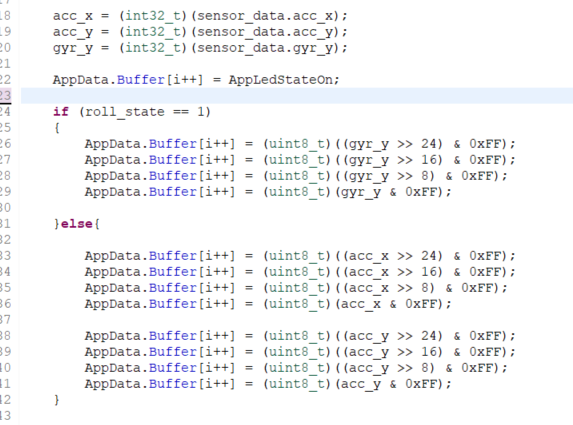
\includegraphics[width=0.9\textwidth]{SendTxData.png}
  \caption{Parte della funzione SendTxData}
  \label{fig:sendtxdata}
\end{figure}
Il primo elemento del buffer (\Verb|AppData.Buffer[0]|) rappresenta lo stato del sistema e da esso dipenderanno i valori acquisiti dai sensori che verranno scritti sul buffer.
  Si utilizza la variabile \Verb|roll_state| per descrivere lo stato della modalità del sistema e il suo valore viene modificato quando l'uC riceve dati dal cloud (Vedi Sezione \ref{sssec:downlink_scheda}):
  \begin{itemize}
    \item \Verb|roll_state| $=1$ indica che la modalità attiva è quella del lancio dei dadi
          \begin{itemize}
            \item il valore di \Verb|gyr_y| sarà scritto negli elementi di \Verb|AppData.Buffer[]| con indice tra 1 e 4.
          \end{itemize}
    \item \Verb|roll_state| $=0$ indica che la modalità attiva è quella di selezione della quantità dei dadi da lanciare
          \begin{itemize}
            \item sul buffer verrano scritti i valori di \Verb|acc_x| e \Verb|acc_y| agli indici 1$\div$4 e 5$\div$8 di \Verb|AppData.Buffer[]| rispettivamente.
          \end{itemize}
  \end{itemize}

  \subsubsection{Downlink scheda}\label{sssec:downlink_scheda}
  % Descrizione della funzione OnRxData:
  % -Riferimento a Variabile roll_state
  % -Lettura del buffer
  % -Accensione del led sulla scheda e cambiamento di stato
  I dati provenienti dal cloud sono processati nella funzione \Verb|OnRxData| (all'interno del file \textit{lora\_app.c} e riportata in Figura \ref{fig:onrxdata}).
  \begin{figure}[h!]
    \centering
    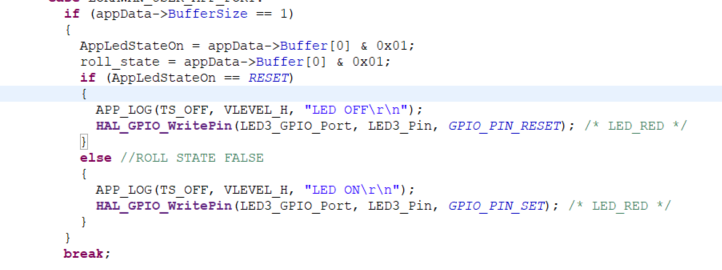
\includegraphics[width=0.9\textwidth]{OnRxData.png}
    \caption{Parte della funzione OnRxData}
    \label{fig:onrxdata}
  \end{figure}
  \\Qui viene letto l'elemento presente all'indice 0 del buffer, il quale indica la modalità di funzionamento del sistema, e viene scritto sulle variabili \Verb|roll_state| e \Verb|AppLedStateOn|. Quest'ultima determina l'accensione o lo spegnimento del LED\_3 della scheda.

